\documentclass[brazil]{article}
\usepackage{graphicx}
\usepackage[T1]{fontenc}
\usepackage[utf8]{inputenc}
\usepackage{lmodern}
\usepackage{babel}
\usepackage{url}

\newcommand{\usd}{US\$}
\newcommand{\brl}{R\$}


\begin{document}


\title{Carta de Pedido de Complemento de Verba para Participação em Evento como Palestrante}

\maketitle

\begin{flushleft}
À Comissão de Graduação do IME/USP,
\end{flushleft}

%\begin{abstract}
%\end{abstract}

Fui aceito para apresentar o artigo ``\emph{A Survey on the Mathematical Emphasis in Brazilian Computer Science Curricula}'' no IEEE Frontiers In Education Conference 2013, como parte do meu projeto de iniciação científica no Projeto Apoio BCC. Para viabilizar a viagem de apresentação do trabalho foi feito um pedido de verba à CG em 13 de março de 2013 através do Programa Pró-Int. Tal pedido foi aceito na reunião de abril e o processo 13.1.559.45.2 encontra-se tramitando no momento na Pró-Reitoria de Graduação.

Porém, de março a agosto houve um aumento vertiginoso da cotação do dólar, de \brl1,95 para valores em torno de \brl2,40 até o momento, sem previsão de estabilização ou de queda. Ainda, a organização do evento revisou para cima o valor cobrado pela inscrição de alunos que são apresentadores de trabalhos. Todos esses fatores contribuíram para tornar a viagem planejada inviável apenas com a verba requisitada anteriormente.

Dessa forma, gostaria de requisitar um complemento de verba para equilibrar financeiramente essa viagem novamente. Os valores e orçamentos encontram-sem anexos. Permaceço à disposição para quaisquer dúvidas.


\vfill

\begin{flushright}
\line(1,0){200}\\
Pedro Paulo Vezzá Campos\\
Projeto Apoio BCC\\
\url{pedrovc@ime.usp.br}\\
(11) 97132-1145
\end{flushright}

\newpage 

\section{Orçamento}
Valores em dólares foram convertidos considerando o câmbio de \usd1,00 = \brl2,50.

\subsection{Inscrição no Evento}
Para estudantes em tempo integral que desejam apenas participar do evento, o FIE2013 estipula uma taxa de inscrição de \usd300,00 (\brl750,00). Porém, houve a decisão que alunos que sejam os únicos a apresentarem um trabalho no evento, como é o caso do artigo em questão, será obrigatória o pagamento da uma taxa de inscrição integral, no valor de \usd500,00 (\brl1250,00). Para este item já foi liberada a quantia de \brl682,50. Será necessária uma complementação no valor de \brl567,50.

\subsection{Passagem Aérea}
Os valores das passagens aéreas flutuaram para baixo de uma maneira a compensar o aumento da cotação do dólar.

\subsection{Hospedagem e traslado}
Verificando valores atualizados no \url{decolar.com} de hospedagens, foi possível encontrar hotéis a um valor médio de \brl165,00 por noite, inclusos taxas e impostos. Já o traslado aeroporto -- hotel e hotel -- centro de convenções, de acordo como site \url{taxifarefinder.com} encontra-se em \usd20,00 por trajeto. No pedido anterior foi requisitada uma quantia de \brl698,90 para cobrir os gastos com 4 pernoites e traslados. O valor atualizado é de \brl1160,00, uma diferença de \brl461,10.

\subsection{Alimentação}
Durante a viagem serão consumidas 6 refeições. Cada uma teve o valor atualizado para \brl30,00 versus \brl19,50 da cotação anterior, uma diferença de \brl10,50.

\subsection{Totais}
\begin{description}
	\item[Inscrição] \brl567,50
	\item[Passagem Aérea] \brl0,00
	\item[Hospedagem e traslado] \brl461,10
	\item[Alimentação] \brl63,00
	\item[Total] \brl1091,60
\end{description}

%\usepackage{graphics} is needed for \includegraphics
\begin{figure}[htp]
\begin{center}
  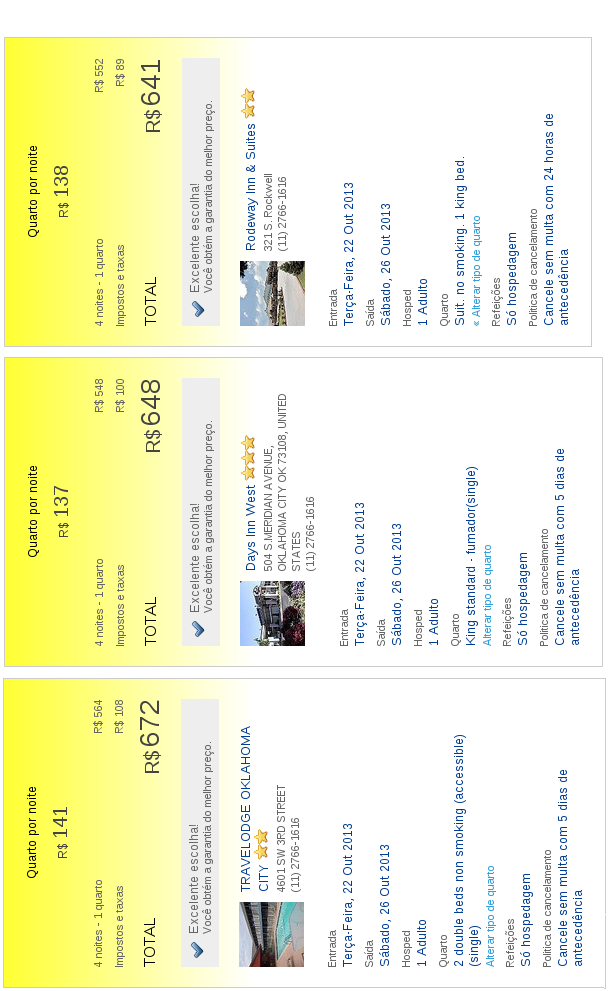
\includegraphics[width=0.9\linewidth]{hoteis.png}
  \caption[Opções de hotéis]{Opções de hotéis}
\end{center}
\end{figure}


\end{document}

